\subsubsection{Devel}
\label{sec:devel}

\paragraph{}
The Devel component provides developer tools for generating new components and processes. All of the actions in this controller require the 'dev' role. It exists as a seperate, installable component and should not be installed in a deployed instance of ROME.

% \begin{scriptsize}
% \begin{verbatim}
% devel/components
% devel/component/current
% devel/component/create
% devel/component/select
% devel/component/update
% devel/component/autocomplete
% devel/process/create
% devel/process/delete
% devel/process/form
% devel/process/accepts_form
% devel/process/creates_form
% devel/process/autocomplete
% devel/process/add_accepts
% devel/process/add_creates
% devel/process/delete_accepts
% devel/process/delete_creates
% devel/datatype/autocomplete
% devel/datatype/description_autocomplete
% devel/datatypes
% devel/datatype/current
% devel/datatype/create
% devel/datatype/delete
% devel/datatype/update
% devel/datatype/select
% devel/component/distribution
% \end{verbatim}
% \end{scriptsize}

\paragraph{}
The controller for the Devel component is ROME::Controller::Devel. This controller provides the functionality to create, select, update and delete components. Processes can be added to and deleted from the selected component. Datatypes a process accepts and creates can be added to and deleted from a process. Parameters can be added to and deleted from a process and constraints defined for those parameters. The process template file that will be used to generate the R script can be uploaded and assigned to the component. For processes which require more complicated controller actions and view templates, the Devel component can be used to provide a skeleton structure that may be fleshed out by the developer. 

\paragraph{}
The url \url{../devel/components} maps to the controller's \texttt{index} action which returns the main component development page. Here, a developer can select an existing component to edit or create a new one. Figure \ref{fig:devel_component} shows the basic default Devel component page. Having created or selected a component, the page is updated with the details of that component and the developer is presented with options to add new processes to the component. Once processes have been added, they will be given the option to add accepted and created datatypes and parameters to that component and to upload a new, or replacement, script template (figures \ref{fig:devel_new_param}, \ref{fig:devel_add_template}). When a new component is created, or a process added to an existing component, the appropriate controller code is generated from templates on the server. To use the new component within ROME the server will require restarting, and the developer will be prompted accordingly. Having generated and tested a new component, the Devel component also provides an option for the developer to package their component for distribution.


\begin{figure}[h]
\centering
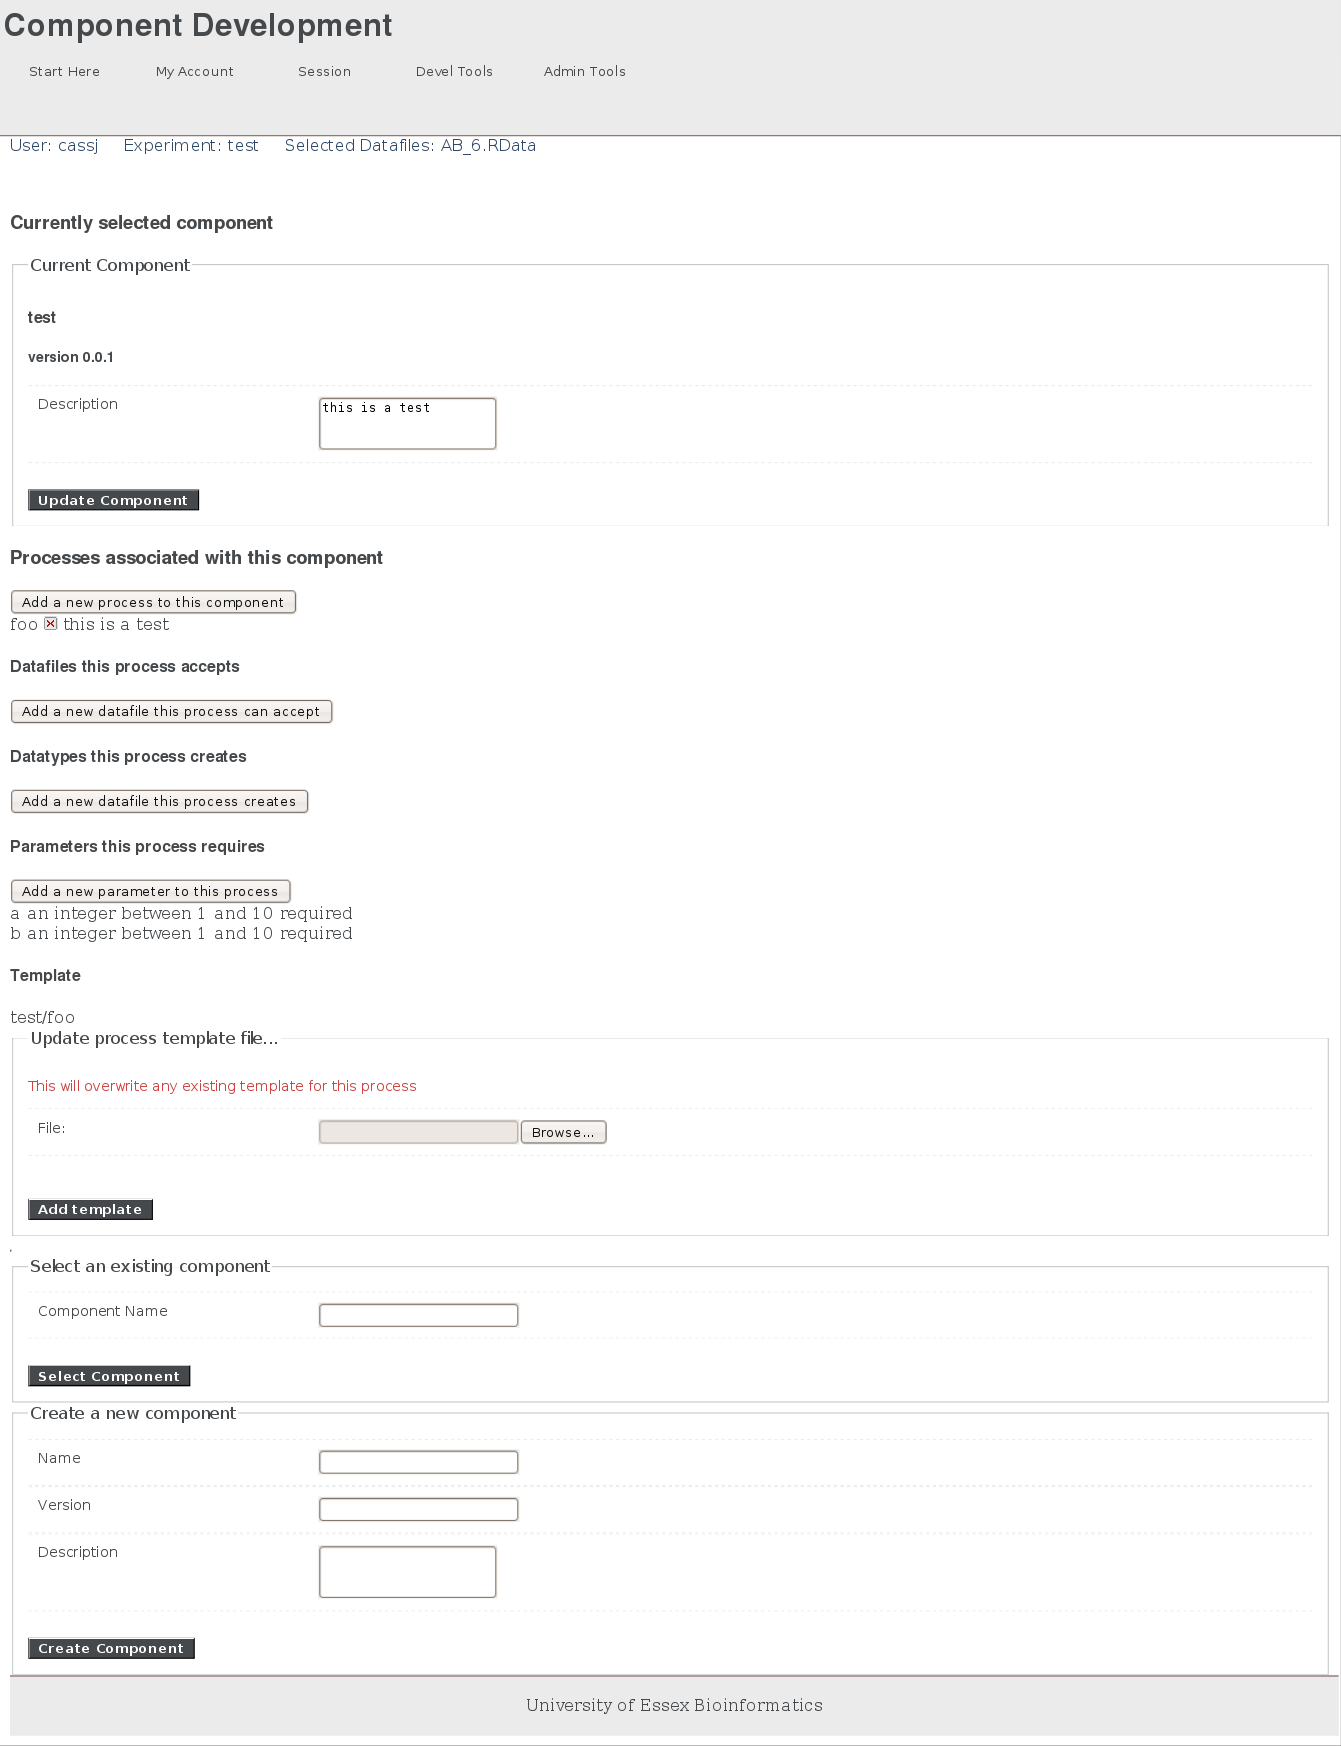
\includegraphics[scale=0.25, ]{../rome/docs/images/screenshots/devel_component}
\caption{The Devel Component Page}\label{fig:devel_component}
\end{figure}
\clearpage

\begin{figure}[h]
\centering
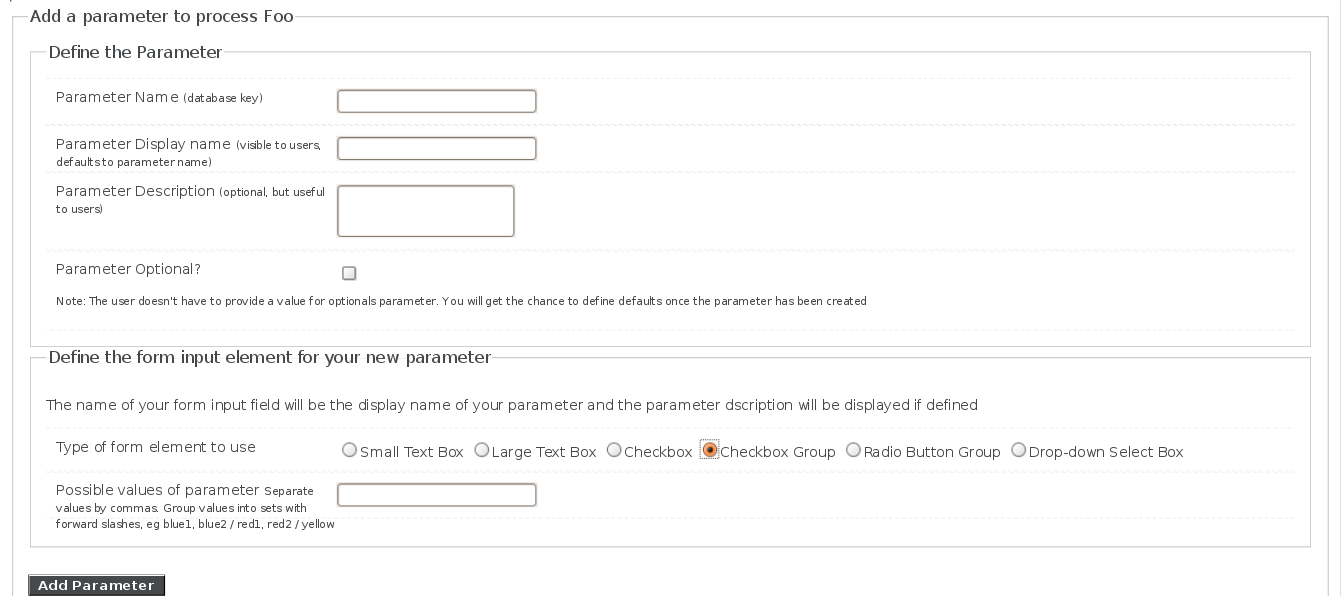
\includegraphics[scale=0.45, angle=90]{../rome/docs/images/screenshots/devel_new_param}
\caption{Adding a Parameter to a Process}\label{fig:devel_new_param}
\end{figure}

\begin{figure}[h]
\centering
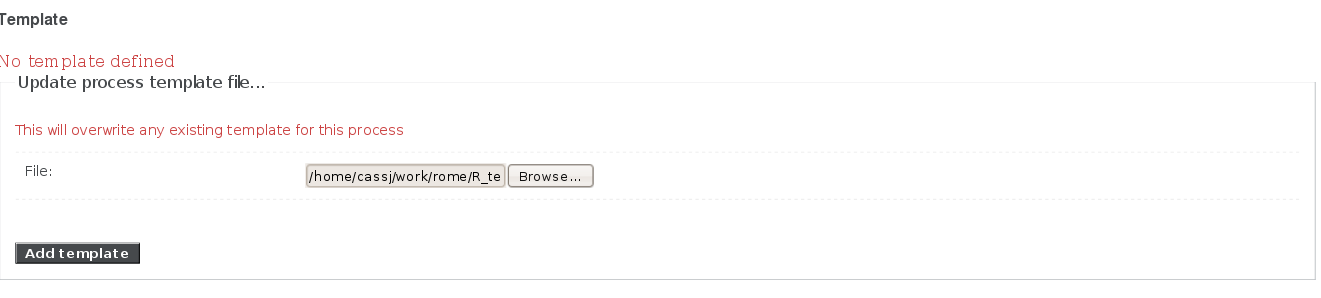
\includegraphics[scale=0.45, angle=90]{../rome/docs/images/screenshots/devel_add_template}
\caption{Adding a Template to a Process}\label{fig:devel_add_template}
\end{figure}
\clearpage

\paragraph{}
As well as providing tools for generating new components, the devel component provides functionality for adding new datatypes to the database. Currently the user may generate as many datatypes as they require, however if multiple developers are producing components this is not a sustainable model. In the future it will make sense to have a central database of datatypes from which the developer can select the one they need. If a new datatype is required, it could then be registered with the central list of datatypes. This will allow components developed by different people to interact as they will have a common set of datatypes.

\paragraph{}
A worked example of developing, distributing, installing and uninstalling a simple component via the Devel component is presented in appendix \ref{sec:comp_dev}
